\begin{figure}[!htb]
  \begin{center}
    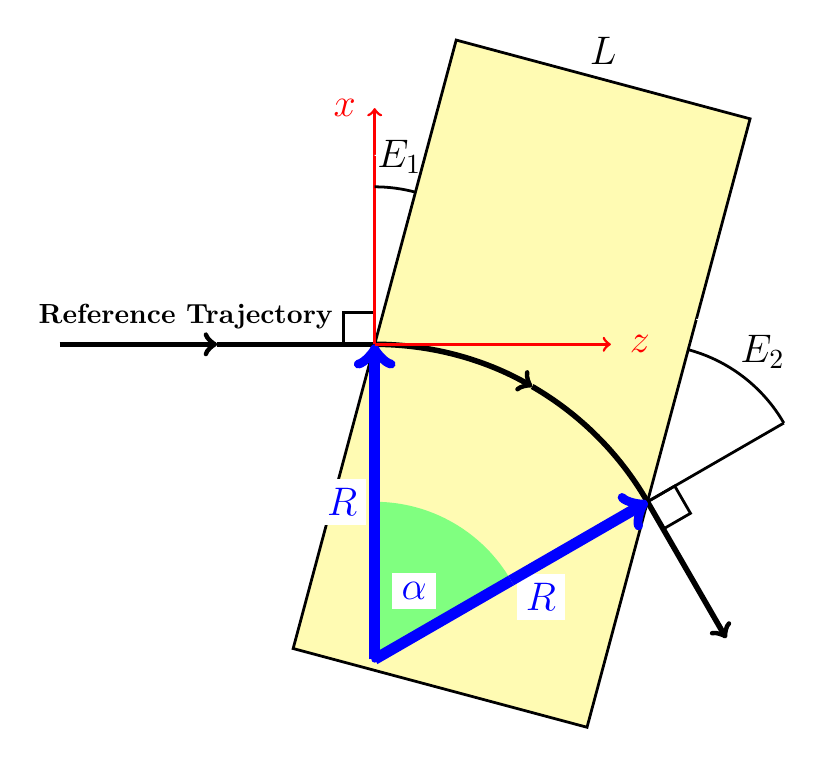
\begin{tikzpicture}[scale=4]
      % First draw rectangular magnet shape.
      \draw[white,rotate around={-15:(0.0,0.0)}] (0.0,1.0) -- (0.4829629,1.0)
      node[above=2pt] {\Large{\textbf{\color{black}$L$}}};
      \filldraw[yellow!30!white,rotate around={-15:(0.0,0.0)}] (0,-1.0) rectangle (0.9659258,1.0);
      \draw[line width=1pt,rotate around={-15:(0.0,0.0)}] (0,-1.0) rectangle (0.9659258,1.0);

      % Now draw squares indicating 90 degree angles to bend radius at entrance and exit.
      \draw[line width=1pt] (0.0,0.0) rectangle (-0.1,0.1);
      \draw[line width=1pt,rotate around={-60:(0.0,-1.0)}]
      (0.0,0.0) rectangle (0.1,0.1);

      % Draw reference particle path.
      \draw[white] (-1.1,0.0) -- (-0.6,0.0)
      node[above=2pt] {\textbf{\color{black}Reference Trajectory}};
      \draw[arrows=->,line width=2pt] (-1.0,0.0) -- (-0.5,0.0);
      \draw[line width=2pt] (-0.5,0.0) -- (0.0,0.0);
      \draw[arrows=->,line width=2pt] (0.0,0.0) arc (90:60:1.0);
      \draw[line width=2pt] (0.5,-0.133975) arc (60:30:1.0);
      \draw[arrows=->,line width=2pt] (0.8660254,-0.5) -- (1.1160254,-0.9330127);

      % Draw bend angle.
      \fill[green!50!white] (0.0,-1.0) -- (0.0,-0.5) arc (90:30:0.5) -- (0.0,-1.0);
      \draw[green!50!white] (0.0,-0.75) arc (90:60:0.25)
      node[fill=white] {\Large{\textbf{\color{blue}$\alpha$}}};

      % Draw bend radii at entrance and exit.
      \draw[blue,line width=4pt] (0.0,-1.0) -- (0.0,-0.5)
      node[blue,left=1pt,fill=white] {\Large{\textbf{$R$}}};
      \draw[arrows=->,blue,line width=4pt] (0.0,-0.5) -- (0.0,0.0);
      \draw[blue,line width=4pt] (0.0,-1.0) -- (0.4330127,-0.75)
      node[below=6pt,right=0pt,fill=white] {\Large{\textbf{$R$}}};
      \draw[arrows=->,blue,line width=4pt] (0.4330127,-0.75) -- (0.8660254,-0.5);
      \filldraw[blue] (0.0,-1.0) circle (0.25pt);

      % Draw reference axes.
      \draw[red,arrows=->,line width=1pt] (0.0,0.0) -- (0.0,0.75) node[left=3pt] {\Large{\textbf{$x$}}};
      \draw[red,arrows=->,line width=1pt] (0.0,0.0) -- (0.75,0.0) node[right=3pt] {\Large{\textbf{$z$}}};

      % Label entrance angle.
      \draw[line width=1pt] (0.0,0.5) arc (90:75:0.5);
      \draw[white] (0.0,0.6) arc (90:82.5:0.6) node[] {\Large{\textbf{\color{black}$E_{1}$}}};

      % Label exit angle.
      \draw[line width=1pt,xshift=0.8660254cm,yshift=-0.5cm,rotate around={-60:(0.0,0.0)}] (0.0,0.0) -- (0.0,0.5);
      \draw[line width=1pt,xshift=0.8660254cm,yshift=-0.5cm,rotate around={-15:(0.0,0.0)}] (0.0,0.5) arc(90:45:0.5);
      \draw[white,xshift=0.8660254cm,yshift=-0.5cm,rotate around={-15:(0.0,0.0)}] (0.0, 0.6) arc (90:67.5:0.6)
      node[] {\Large{\textbf{\color{black}$E_{2}$}}};

    \end{tikzpicture}
  \end{center}
  \caption{Illustration of a general rectangular bend (\keyword{RBEND}) with a positive bend angle $\alpha$. The
    entrance edge angle, $E_{1}$, is positive in this example. An \keyword{RBEND} has parallel entrance and exit
    pole faces, so the exit angle, $E_{2}$, is uniquely determined by the bend angle, $\alpha$, and $E_{1}$
    ($E_{2}=\alpha - E_{1}$). For a positively charge particle, the magnetic field is directed out of the page.}
  \label{fig:rbend}
\end{figure}